\documentclass[oneside,numbers,spanish]{ezthesis}
%% # Opciones disponibles para el documento #
%%
%% Las opciones con un (*) son las opciones predeterminadas.
%%
%% Modo de compilar:
%%   draft            - borrador con marcas de fecha y sin im'agenes
%%   draftmarks       - borrador con marcas de fecha y con im'agenes
%%   final (*)        - version final de la tesis
%%
%% Tama'no de papel:
%%   letterpaper (*)  - tama'no carta (Am'erica)
%%   a4paper          - tama'no A4    (Europa)
%%
%% Formato de impresi'on:
%%   oneside          - hojas impresas por un solo lado
%%   twoside (*)      - hijas impresas por ambos lados
%%
%% Tama'no de letra:
%%   10pt, 11pt, o 12pt (*)
%%
%% Espaciado entre renglones:
%%   singlespace      - espacio sencillo
%%   onehalfspace (*) - espacio de 1.5
%%   doublespace      - a doble espacio
%%
%% Formato de las referencias bibliogr'aficas:
%%   numbers          - numeradas, p.e. [1]
%%   authoryear (*)   - por autor y a'no, p.e. (Newton, 1997)
%%
%% Opciones adicionales:
%%   spanish         - tesis escrita en espa'nol
%%
%% Desactivar opciones especiales:
%%   nobibtoc   - no incluir la bibiolgraf'ia en el 'Indice general
%%   nofancyhdr - no incluir "fancyhdr" para producir los encabezados
%%   nocolors   - no incluir "xcolor" para producir ligas con colores
%%   nographicx - no incluir "graphicx" para insertar gr'aficos
%%   nonatbib   - no incluir "natbib" para administrar la bibliograf'ia

%% Paquetes adicionales requeridos se pueden agregar tambi'en aqu'i.
%% Por ejemplo:
%\usepackage{subfig}
%\usepackage{multirow}
\usepackage[utf8]{inputenc}

%% # Datos del documento #
%% Nota que los acentos se deben escribir: \'a, \'e, \'i, etc.
%% La letra n con tilde es: \~n.

\author{Efrain Tlapale Pulido}
\title{Desarrollo de una guía para la transferencia de conocimiento de la arquitectura SOA a empleados de nuevo ingreso de la empresa MBN}
\degree{Ingeniero en Sistemas Computacionales}
\supervisor{Nombre de mi Asesor}
\institution{Universidad del Valle de Tlaxcala}

%% # M'argenes del documento #
%% 
%% Quitar el comentario en la siguiente linea para austar los m'argenes del
%% documento. Leer la documentaci'on de "geometry" para m'as informaci'on.

%\geometry{top=40mm,bottom=33mm,inner=40mm,outer=25mm}

%% El siguiente comando agrega ligas activas en el documento para las
%% referencias cruzadas y citas bibliogr'aficas. Tiene que ser *la 'ultima*
%% instrucci'on antes de \begin{document}.
\hyperlinking
\begin{document}

%% En esta secci'on se describe la estructura del documento de la tesis.
%% Consulta los reglamentos de tu universidad para determinar el orden
%% y la cantidad de secciones que debes de incluir.

%% # Portada de la tesis #
%% Mirar el archivo "titlepage.tex" para los detalles.
%% ## Construye tu propia portada ##
%% 
%% Una portada se conforma por una secuencia de "Blocks" que incluyen
%% piezas individuales de informaci'on. Un "Block" puede incluir, por
%% ejemplo, el t'itulo del documento, una im'agen (logotipo de la universidad),
%% el nombre del autor, nombre del supervisor, u cualquier otra pieza de
%% informaci'on.
%%
%% Cada "Block" aparece centrado horizontalmente en la p'agina y,
%% verticalmente, todos los "Blocks" se distruyen de manera uniforme 
%% a lo largo de p'agina.
%%
%% Nota tambi'en que, dentro de un mismo "Block" se pueden cortar
%% lineas usando el comando \\
%%
%% El tama'no del texto dentro de un "Block" se puede modificar usando uno de
%% los comandos:
%%   \small      \LARGE
%%   \large      \huge
%%   \Large      \Huge
%%
%% Y el tipo de letra se puede modificar usando:
%%   \bfseries - negritas
%%   \itshape  - it'alicas
%%   \scshape  - small caps
%%   \slshape  - slanted
%%   \sffamily - sans serif
%%
%% Para producir plantillas generales, la informaci'on que ha sido inclu'ida
%% en el archivo principal "tesis.tex" se puede accesar aqu'i usando:
%%   \insertauthor
%%   \inserttitle
%%   \insertsupervisor
%%   \insertinstitution
%%   \insertdegree
%%   \insertfaculty
%%   \insertdepartment
%%   \insertsubmitdate

\begin{titlepage}
  \TitleBlock{\scshape\insertinstitution}
  \TitleBlock{\Huge\scshape\inserttitle}
  \TitleBlock{\scshape
    Tesis presentada por \insertauthor \\
    para obtener el grado de \insertdegree}
  \TitleBlock{\insertsubmitdate}
\end{titlepage}

%% Nota 1:
%% Se puede agregar un escudo o logotipo en un "Block" como:
%%   \TitleBlock{\includegraphics[height=4cm]{escudo_uni}}
%% y teniendo un archivo "escudo_uni.pdf", "escudo_uni.png" o "escudo_uni.jpg"
%% en alg'un lugar donde LaTeX lo pueda encontrar.

%% Nota 2:
%% Normalmente, el espacio entre "Blocks" se extiende de modo que el
%% contenido se reparte uniformemente sobre toda la p'agina. Este
%% comportamiento se puede modificar para mantener fijo, por ejemplo, el
%% espacio entre un par de "Blocks". Escribiendo:
%%   \TitleBlock{Bloque 1}
%%   \TitleBlock[\bigskip]{Bloque2}
%% se deja un espacio "grande" y de tama~no fijo entre el bloque 1 y 2.
%% Adem'as de \bigskip est'an tambi'en \smallskip y \medskip. Si necesitas
%% aun m'as control puedes usar tambi'en, por ejemplo, \vspace*{2cm}.




%% # Prefacios #
%% Por cada prefacio (p.e. agradecimientos, resumen, etc.) crear
%% un nuevo archivo e incluirlo aqu'i.
%% Para m'as detalles y un ejemplo mirar el archivo "gracias.tex".
%% Las secciones del "prefacio" inician con el comando \prefacesection{T'itulo}
%% Este tipo de secciones *no* van numeradas, pero s'i aparecen en el 'indice.
%%
%% Si quieres agregar una secci'on que no vaya n'umerada y que *tampoco*
%% aparesca en el 'indice, usa entonces el comando \chapter*{T'itulo}
%%
%% Recuerda que aqu'i ya puedes escribir acentos como: 'a, 'e, 'i, etc.
%% La letra n con tilde es: 'n.

\prefacesection{Agradecimientos}

Gracias a mi familia, al Maestro Roberto Capistran, a MBN y al PhD Alberto Portilla

%% Por si alguien tiene curiosidad, este "simp'atico" agradecimiento est'a
%% tomado de la "Tesis de Lydia Chalmers" basada en el universo del programa
%% de televisi'on Buffy, la Cazadora de Vampiros.
%% http://www.buffy-cazavampiros.com/Spiketesis/tesis.inicio.htm


%% # 'Indices y listas de contenido #
%% Quitar los comentarios en las lineas siguientes para obtener listas de
%% figuras y cuadros/tablas.
\tableofcontents
%\listoffigures
%\listoftables

%% # Cap'itulos #
%% Por cada cap'itulo hay que crear un nuevo archivo e incluirlo aqu'i.
%% Mirar el archivo "intro.tex" para un ejemplo y recomendaciones para
%% escribir.
%% Los cap'itulos inician con \chapter{T'itulo}, estos aparecen numerados y
%% se incluyen en el 'indice general.
%%
%% Recuerda que aqu'i ya puedes escribir acentos como: 'a, 'e, 'i, etc.
%% La letra n con tilde es: 'n.

\chapter{Introducci'on}

MBN es una empresa dedicada a proporcionar consultoría de negocios y desarrollo de software enfocada en apoyar a las organizaciones que requieren la adopción de tecnologías de información como estrategia para acelerar su crecimiento, facilitando la optimización y simplificación de su proceso de negocio.

Esta empresa desarrolla sistemas de información modernos, por lo que deben considerar aspecto como alta disponibilidad, rendimiento, portabilidad,separación de intereses, y facilidad de mantenimiento. Según los requerimientos antes mencionados, se desarrollan sistemas de información distribuidos bajo la arquitectura SOA (Service Oriented Architecture o Arquitectura Orientada a Servicios), este modelo permite separar las capas de la aplicación creando subsistemas independientes que se unifican para lograr una plataforma completa. 

La abstracción en capas de un sistema mejora aspectos organizacionales en el desarrollo de un proyecto, pero genera problemas si no se definen y especifican todos los componentes que conforman la arquitectura, tal es el caso de MBN, pues no se cuenta con una arquitectura defina para los sistemas que desarrollan. 

La arquitectura de los sistemas desarrollados debe ser entendida y adoptada por todos los miembros involucrados en el proceso, debido a que no se cuenta con una bien establecida, el proceso de adopción y de transferencia del conocimiento no se lleva a cabo de manera eficiente,  en ocasiones prolongándose hasta 8 meses, lo cual consume recursos y genera retrasos que una empresa de alto nivel como MBN no se puede permitir.

\section{ Planteamiento del Problema }
La empresa Miracle Bussines Network no cuenta con una arquitectura estandarizada para el desarrollo de sistemas de información, por lo que se complica el proceso de construcción de software así como el de transferencia de conocimiento.

\section{ Estado del Arte }

\subsection{ Sistemas de información distribuidos }

Los sistemas de información han evolucionado de acuerdo a las necesidades generadas a partir de avances tecnológicos empleados en la construcción de hardware y software. Los sistemas de información siempre se han podido abstraer en 3 capas: presentación, lógica y administración de recursos.
Los primeros sistemas de información mantenían las 3 capas antes mencionadas en una sola computadora, por lo que eran consideradas aplicaciones monolíticas, esto producía componentes fuertemente acoplados que no podían ser utilizados en ambientes externos

Con la aparición de la red de área local, comenzó una separación de capas que distribuía procesos en diferentes computadoras, la capa de presentación se designo exclusivamente a los clientes y la de lógica y recursos a los servidores. Muchos estilos arquitectónicos se crearon basándose en esta separación de capas.
Cuando el avance en la teoría de redes de computadoras logró aumentar el ancho de banda disponible, los sistemas de información comenzaron a aislar las capas y se logró una completa distribución, se creó una capa extra entre el cliente y el servidos llamada “middleware”, que permitía comunicar todas las capas entre sí y mantener organizado el flujo de información.

\begin{figure}[H]
  \begin{center}
    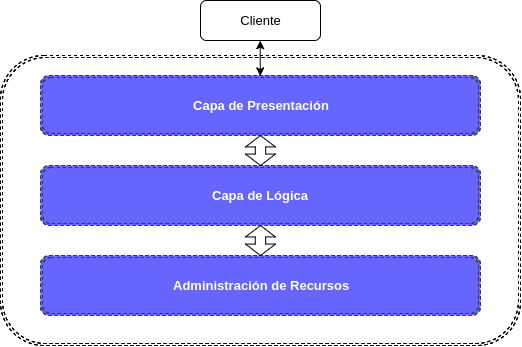
\includegraphics[scale=0.8]{DistArch}
  \end{center}
  \caption{Arquitectura de un Sistema Distribuido}
\end{figure}

\subsection{ Arquitecturas distribuidas modernas }
Como se mencionó en el punto anterior, los sistemas de información modernos utilizan estilos arquitectónicos distribuidos para mejorar el rendimiento, construcción y mantenimiento. A continuación se presentan las principales arquitecturas distribuidas: 

\subsubsection{ Cliente-Servidor }
Esta arquitectura distribuida reparte los requerimientos de procesamiento entre dos entidades, una que brinda servicios y recursos, llamada servidor y una que solicita esos servicios, llamada cliente.
Una de las principales ventajas de esta arquitectura no se refiere al rendimiento del sistemas sino a que permite una separación de responsabilidades y un esquema centralizado de las capas que lo conforman. Esta arquitectura permite a las organizaciones mantener un control sobre los equipos de trabajo que interfieren en la construcción de software, pues los equipos se dedican exclusivamente a modificar una parte del sistema. Si los equipos no mantienen un estándar ni expresan correctamente las especificaciones de la capa que desarrollan, el sistema puede tener problemas de integración.

\subsubsection{ N-Capas }
 Las arquitecturas a n-capas (también referenciadas como tiers, tercios o niveles) se presenta como una extensión al modelo clásico de 3 capas. En esta arquitectura se vinculan múltiples subsistemas creados debido a la complejidad que las capas pueden adquirir, por ejemplo, la capa de recursos tradicionalmente consiste en un sistema de base de datos, esta puede ser sustituida por un sistema de dos o tres capas donde se centralicen varias BD. Otra capa que se puede extender es la de presentación. Para distribuir eficientemente los procesos del sistema se puede implementar un servidor web encargado de generar las páginas html solicitadas por los clientes.
Conforme se van añadiendo más capas a los sistemas de información también se hace más complejo su desarrollo, mantenimiento y gestión.

\subsubsection{ SOA }
La arquitectura SOA (Service Ortented Architecture) es utilizada para crear sistemas distribuidos, permite una alineación directa de los procesos o lógica de negocio de las organizaciones con las funciones que ofrecen los sistemas desarrollados. Este tipo de sistemas permite una alta escalabilidad al  abstraer la lógica de negocios en Servicios. Los servicios son interfaces, por lo que no se describe la tecnología ni el funcionamiento interno de estos, sino que describen el comportamiento. Por lo regular  los servicios de una arquitectura SOA se implementan como WebServices, los cuales son un conjunto de tecnologías utilizadas para transferir datos entre aplicaciones a través de Internet, pueden utilizar distintos estándares, como XML, REST, etc.
Los servicios web en una arquitectura SOA permiten tener bien definida la manera en que se exponen y consumen los servicios, por lo que la integración de todas las capas del sistema se estandariza y facilita.

\subsection{ Transferencia de conocimiento en MBN }
En la empresa MBN actualmente la transferencia de conocimiento respecto a la arquitectura de las sistemas de información que desarrollan se lleva a cabo de manera genérica, pues se da un panorama amplio de cómo está conformada la arquitectura, pero no se cuenta con una guía institucional que cubra aspectos como: configurar el ambiente de desarrollo, comprobar que el ambiente de desarrollo se ejecute correctamente y desarrollar un proyecto integrador para familiarizarse con las tecnologías utilizadas.Según estudios internos la transferencia de conocimientos básicos sobre la arquitectura de aplicaciones de MBN requiere de 4 a 8 meses.

\section{ Justificación }
Para que un sistema de información SOA se pueda desarrollar sin inconvenientes, es necesario que todos los involucrados adopten la arquitectura y conozcan todos los componentes que la integran.
La propuesta de una arquitectura formal para los sistemas desarrollados en MBN optimizará el tiempo requerido para adoptarla, también facilitará una de las partes más importantes dentro de una empresa de  TI: la transferencia de conocimiento. 

\section{ Objetivos }
El objetico general de esta tesis es desarrollar una propuesta de arquitectura SOA para los sistemas de información desarrollados en MBN
Para alcanzar el objetivo general se plantean los siguientes objetivos específicos:
\begin{itemize}
\item Analizar y caracterizar las principales tecnologías utilizadas en los sistemas ya desarrollados por MBN.
\item Documentar la propuesta de Arquitectura 
\item Elaborar un documento formal que facilite la adopción de la arquitectura de MBN
\end{itemize}
\chapter{ Marco Teórico }

\section{ Arquitectura SOA }
SOA es una arquitectura de software distribuida orientada a servicios, en esta toda la lógica de negocio del sistema se divide en unidades elementales llamadas servicios, los cuales representan una parte del flujo de información en un sistema.
Los servicios pueden tener diferentes implementaciones, pero la más común y eficiente son los Servicios Web (Web Services).

\section{ Servicios Web }
Un servicio web es un programa independiente que representa un proceso dentro de la lógica de negocio de un sistema con interfaces abiertas utilizando protocolos de Internet.

La descripción de un servicio web involucra los siguientes elementos:

\begin{itemize}
\item Lenguaje base en común. Se debe considerar la adopción de un lenguaje base para transmitir los datos que el servicio web exponga o reciba, durante años el estándar más utilizado era XML, pero JSON ha sobresalido en años recientes por ser un formato más ligero y fácil de entender, lo que mejora el rendimiento y universalidad de los servicios.
\item  Interfaces. Es necesario definir de manera correcta la interfaz de los servicios web, pues se debe indicar el URI y el protocolo con el que se obtiene acceso al servicio, los datos que requiere y los datos que regresan.
\item Protocolos de Negocio. En ocasiones para completar una operación requiere llamar a varios servicios para ser completada, por lo que es importante definir qué servicios y en qué orden se llaman.
\item Propiedades. Las propiedades pueden representar características no funcionales de los servicios, por ejemplo una descripción textual del servicio o la versión del mismo.
\end{itemize}


Para definir la estructura de los servicios web se deben considerar dos aspectos, primero que son una forma de exponer funcionamiento interno de un sistema a clientes externos, y segundo que son aplicaciones independientes y llevan a cabo procesos internos.
\begin{itemize}
\item 
\end{itemize}

\subsection{ Estructura interna de un servicio Web }
La estructura interna de un servicio web puede definirse en 4 aspectos clave 


\subsection{ Estructura externa de un Servicio Web }



\section{ Java }
\section{ Java EE }
\section{ Spring }
Spring es un framework para para la construcción aplicaciones web desarrollado sobre Java EE. Es una de las implementaciones web de Java más utilizadas en la industria, por lo tanto, una de las más estables y eficientes. Spring permite  
\section{json}
\section{PostgreSQL}
\section{ORM}
\section{Hibernate}
\section{Java Server Faces}
\section{PrimeFaces}
\section{WildFly}
%\include{capitulo1}
%\include{capitulo2}
%\include{capitulo3}
%\include{conclu}

\appendix
%% Cap'itulos incluidos despues del comando \appendix aparecen como ap'endices
%% de la tesis.
%\include{apendiceA}
%\include{apendiceB}
%\include{apendiceC}

%% Incluir la bibliograf'ia. Mirar el archivo "biblio.bib" para m'as detales
%% y un ejemplo.
\bibliography{biblio}

\end{document}
